\section{Bases de datos en la actualidad}

Se dice que vivimos actualmente en la era de la información. La oración anterior nos hace pensar un poco en la importancia que tiene la información (o datos) hoy en día, y de la importancia que tiene la preservación de esta información, así como su acceso rápido y eficiente.Todos estos inconvenientes y estas necesidades se pueden resolver con la implementación de bases de datos \cite{ref6}.

Hoy en día podemos hablar sobre dos principales modelos de bases de datos: el modelo \texttt{SQL} y \texttt{NoSQL}.

\begin{figure}[H]
	\centering
	\begin{subfigure}[b]{0.4\textwidth}
		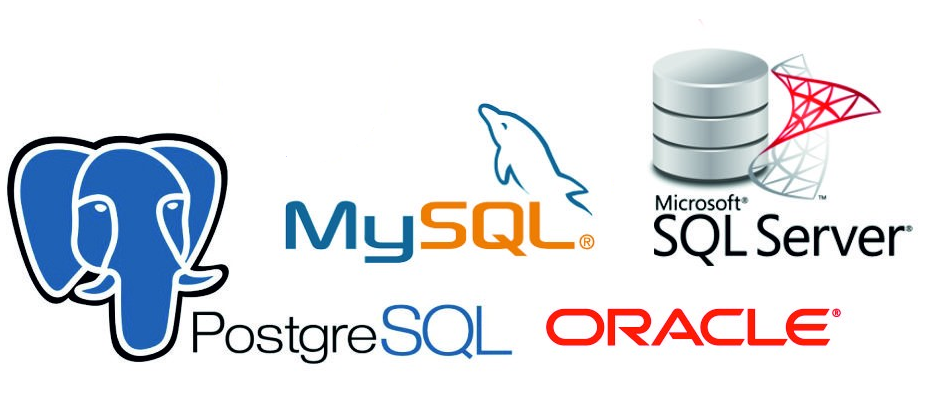
\includegraphics[width=\textwidth,height=90px]{images/sql}
		\caption{SQL}
		\label{fig:sql}
	\end{subfigure}
	~ 
	\begin{subfigure}[b]{0.4\textwidth}
		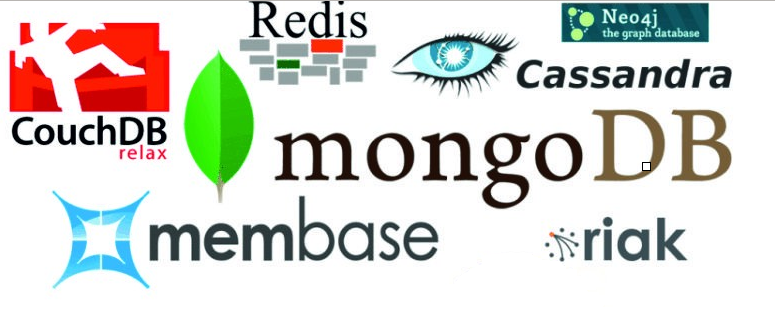
\includegraphics[width=\textwidth,height=90px]{images/nosql}
		\caption{NoSQL}
		\label{fig:nosql}
	\end{subfigure}
	~ 
	\begin{subfigure}[b]{0.5\textwidth}
		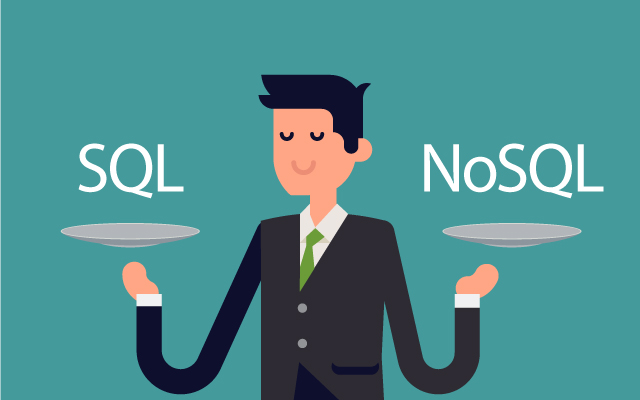
\includegraphics[width=\textwidth,height=90px]{images/sql_o_nosql}
		\caption{¿Cuál elegir?}
		\label{fig:cualelegir}
	\end{subfigure}
\end{figure}

En las siguientes secciones, se detallarán más en profundidad cómo funcionan las bases de datos SQL y NoSQL, y en qué contextos de uso es más apropiado utilizar una u otra.

\newpage